\documentclass[conference,letterpaper,10pt]{IEEEtran}
\IEEEoverridecommandlockouts

\usepackage[T1]{fontenc}
\usepackage[utf8]{inputenc}
\usepackage{cite}
\usepackage{amsmath,amssymb}
\usepackage{graphicx}
\usepackage{booktabs}
\usepackage{colortbl}   % bands the trigger table's middle group
\usepackage{algorithm}
\usepackage{algorithmic}
\usepackage{url}
\usepackage[hidelinks]{hyperref}
\hypersetup{pdftitle={An Empirical Evaluation of TLS Fingerprint-Based Filtering for Application-Layer DDoS},
  pdfauthor={Natanael Oliveira, Arthur Kobielski, Marcos Luna, Luigi Carro, J\'eferson Campos Nobre, Eder John Scheid},
  pdfkeywords={security management, application-layer DDoS, mitigation policy, TLS fingerprinting, statistical calibration, collateral damage}}


\renewcommand{\topfraction}{0.92}
\renewcommand{\dbltopfraction}{0.92}
\renewcommand{\bottomfraction}{0.6}
\renewcommand{\textfraction}{0.07}
\renewcommand{\floatpagefraction}{0.75}
\renewcommand{\dblfloatpagefraction}{0.75}
\setcounter{topnumber}{4}
\setcounter{dbltopnumber}{1}
\setcounter{totalnumber}{5}
\setcounter{bottomnumber}{2}
\setlength{\textfloatsep}{10pt plus 2pt minus 2pt}
\setlength{\intextsep}{8pt plus 2pt minus 2pt}
\setlength{\dbltextfloatsep}{10pt plus 2pt minus 2pt}

%% Code blocks are floats with their own counter (Listing 1), so they leave no
%% gaps in the numbering of the image figures (Figs. 1-4).
\usepackage{float}
\usepackage{stfloats}
%% Caption style matching IEEEtran's figures ("Listing 1. Text"): float.sty's
%% plain style omits the separating period.
\makeatletter
\newcommand\floatc@ieeelst[2]{\setbox\@tempboxa\hbox{\footnotesize #1.\enskip #2}%
  \ifdim\wd\@tempboxa>\hsize \footnotesize #1.\enskip #2\par
  \else \hbox to\hsize{\hfil\box\@tempboxa\hfil}\fi}
\newcommand\fs@ieeelst{\def\@fs@cfont{\footnotesize}\let\@fs@capt\floatc@ieeelst
  \def\@fs@pre{}\def\@fs@mid{\vspace\abovecaptionskip}\def\@fs@post{}%
  \let\@fs@iftopcapt\iffalse}
\makeatother
\floatstyle{ieeelst}
\newfloat{listing}{tbp}{lol}
\floatname{listing}{Listing}

\newcommand{\ie}{\textit{i}.\textit{e}.,\ }
\newcommand{\eg}{\textit{e}.\textit{g}.,\ }
\newcommand{\cf}{\textit{c}\textit{f}.\ }
\newcommand\1{\textit{(i)}}
\newcommand\2{\textit{(ii)}}
\newcommand\3{\textit{(iii)}}
\newcommand\4{\textit{(iv)}}
\newcommand\5{\textit{(v)}}
\newcommand\6{\textit{(vi)}}
\newcommand\7{\textit{(vii)}}
\newcommand\8{\textit{(viii)}}
\newcommand\9{\textit{(ix)}}

\newcommand\itemA{\textit{(a)}}
\newcommand\itemB{\textit{(b)}}
\newcommand\itemC{\textit{(c)}}
\newcommand\itemD{\textit{(d)}}
\newcommand\itemE{\textit{(e)}}


\IfFileExists{pcrr8t.tfm}{}{\renewcommand{\ttdefault}{lmtt}}

\def\BibTeX{{\rm B\kern-.05em{\sc i\kern-.025em b}\kern-.08em T\kern-.1667em\lower.7ex\hbox{E}\kern-.125emX}}

\begin{document}

\title{An Empirical Evaluation of TLS Fingerprint-Based Filtering for Application-Layer DDoS}

\author{\IEEEauthorblockN{Natanael Oliveira\IEEEauthorrefmark{1}, Arthur Kobielski, Marcos Luna,
Luigi Carro, J\'eferson Campos Nobre, and Eder John Scheid}
\IEEEauthorblockA{Institute of Informatics, Universidade Federal do Rio Grande do Sul (UFRGS), Porto Alegre, Brazil\\
\IEEEauthorrefmark{1}Also with Azion Technologies, Brazil\\
\texttt{\{natanael.oliveira, arthur.kobielski, marcos.luna, carro, jcnobre, ejscheid\}@inf.ufrgs.br}}}

\maketitle

\begin{abstract}
TLS fingerprints offer a way to identify application-layer DDoS bots across IP addresses, but their overlap with legitimate clients makes indiscriminate blocking unsafe. We investigate endpoint-relative fingerprint filtering, which uses traffic profiles presumed attack-free to select fingerprints that are unseen at an endpoint or over-represented during a surge, behind a volume trigger and a label-free calibration that targets a false-alarm budget. In a pre-registered two-week evaluation on production CDN endpoints, the scope alone covered about $90\%$ of a 300-bot botnet on new fingerprints at the busiest endpoint, but behind the trigger it covered $3\%$. False alarms were rare, yet the median one would have blocked $39\%$ of its window's legitimate clients, and the fallback exposed far more clients than the filters did. In an exploratory replay of two real, previously mitigated attacks, filters applied one window late would have removed $36\%$ of each attack's requests, with at most $1.6\%$ collateral under two attacker labelings. Fingerprint filters should therefore be judged, at each endpoint, by coverage behind the trigger, damage per false alarm, and fallback exposure.
\end{abstract}


\begin{IEEEkeywords}
security management, application-layer DDoS, mitigation policy, TLS
fingerprinting, collateral damage
\end{IEEEkeywords}



\section{Introduction}
\label{sec:intro}

Application-layer DDoS mitigation remains a problem of both scale and selectivity. In the third quarter of 2026 alone, one CDN provider mitigated 14.4 trillion HTTP DDoS requests~\cite{cloudflare2026q3ddos}. Beyond detecting an attack, mitigation systems must decide which clients to block while preserving legitimate access. Blocking too broadly excludes legitimate users, whereas blocking too narrowly allows attack traffic to reach the service~\cite{soldo2012filtering,dietzel2018stellar}.

Existing mitigation approaches either detect attacks without identifying which clients to block~\cite{tripathi2021application,belcastro2025klage} or select traffic based on source addresses and header fields~\cite{soldo2012filtering,mahajan2002pushback,alcoz2022accturbo}. However, distributed bots can evade address-based rate limits while collectively exhausting a server~\cite{cambiaso2013slowdos}. TLS fingerprinting offers an alternative basis for client selection. A fingerprint such as JA4 summarizes characteristics of the TLS ClientHello, reflecting the client's TLS implementation and configuration rather than its network address. Since botnets may comprise many devices running a relatively small set of TLS implementations, their traffic can concentrate on a limited number of fingerprints. 

However, TLS fingerprints are not exclusive to malicious clients. Legitimate applications using the same TLS implementation can share identical fingerprints~\cite{anderson2019tls}. Consequently, a fingerprint that is prevalent among attack traffic may also be common among legitimate clients. This overlap makes fingerprint-based filtering challenging: selecting fingerprints associated with an attack does not necessarily distinguish malicious clients from legitimate ones.

To evaluate TLS fingerprint-based filtering, we compare the fingerprints observed during an alarm with each endpoint's normal traffic profile, selecting those that are either new or statistically over-represented. This approach draws on anomaly extraction techniques for flow features~\cite{silveira2010urca,brauckhoff2009extraction} and packet attributes~\cite{kim2006packetscore}. Although commercial bot-management platforms already aggregate JA4 signals~\cite{martinetti2024ja4signals}, their effectiveness and collateral costs for client filtering remain insufficiently characterized. We therefore assess their attack coverage, exposure of legitimate traffic, and sensitivity to endpoint characteristics and volume triggers.


Our pipeline operates independently at each endpoint in five-minute windows (\cf Figure~\ref{fig:pipeline}). A volume trigger identifies windows with unusually many clients, and a subsequent \textit{scope} selects fingerprints that are new to the endpoint (\textit{novelty rule}) or over-represented relative to normal traffic (binomial test). If none are selected, a fallback challenges or rate-limits all clients. We calibrate the binomial test on unlabeled, attack-free days to target a $1\%$ false-alarm budget. We evaluate the pipeline offline using generated campaigns, four CDN endpoints, and two real attacks. For the endpoints, we pre-register a 14-day evaluation before examining its data. The evaluation reveals three important findings:

\begin{itemize}
    \item \textit{The volume trigger limits end-to-end coverage.}
    For a 300-bot campaign using new fingerprints, novelty filtering alone covered about $90\%$ of bots, but the complete pipeline covered only $3\%$ (Sections~\ref{sec:symbolic-detector} and~\ref{sec:trigger}).

    \item \textit{Low false-alarm rates can conceal collateral damage.}
    Although filters were selected in only $0.19\%$ of clean windows, the median selection would have blocked $39\%$ of legitimate clients in its window (Section~\ref{sec:posthoc}).

    \item \textit{Fallback mitigation adds substantial exposure.}
    The fallback challenged or rate-limited more legitimate clients than the fingerprint filters blocked (Sections~\ref{sec:posthoc} and~\ref{sec:discussion}).
\end{itemize}

The remainder of this paper is organized as follows.
Section~\ref{sec:rw} reviews the related work. Section~\ref{sec:approach} describes the fingerprint-scoping approach. Section~\ref{sec:method} details the evaluation methodology. Section~\ref{sec:results} reports the evaluation results. Section~\ref{sec:discussion} discusses the findings and limitations, and Section~\ref{sec:conclusion} concludes the paper.

%% ====================================================================
%% ====================================================================
\section{Related Work}
\label{sec:rw}



\begin{table*}[t]
\centering
\caption{Representative approaches and their main focus}
\label{tab:related}
\scriptsize
\setlength{\tabcolsep}{3pt}
\begin{tabular*}{\textwidth}{@{\extracolsep{\fill}}llll@{}}
\toprule
\textbf{Work} & \textbf{Selection} & \textbf{Evaluated on} & \textbf{Main question} \\
\midrule
Attack detectors~\cite{kemp2023approach,belcastro2025klage} & None: an attack verdict & Labeled datasets & Is this traffic an attack? \\
Aggregate filters~\cite{mahajan2002pushback,alcoz2022accturbo,soldo2012filtering} & Header-field aggregates or source prefixes & Simulation and testbeds & Which aggregates or prefixes to limit? \\
Anomaly extraction~\cite{silveira2010urca,brauckhoff2009extraction} & Over-represented feature values & Backbone traces & Which values explain an anomaly? \\
PacketScore~\cite{kim2006packetscore} & Packets scored against a nominal profile & Trace-driven simulation & Which packets to drop under overload? \\
JA3 report~\cite{kobayashi2024ja3} & HTTPS traffic using JA3 & A security operations center & Can JA3 mitigate HTTPS floods? \\
Anti-bot evaluations~\cite{aminazad2020webrunner,vastel2020fpcrawlers} & None: bot detection is tested & Commercial services, live websites & How do bots evade detection? \\
This work & New or over-represented JA4 at the endpoint & Production endpoints, injected and real attacks & What coverage and collateral does filtering yield? \\
\bottomrule
\end{tabular*}
\end{table*}

\begin{figure*}[t]
\centering
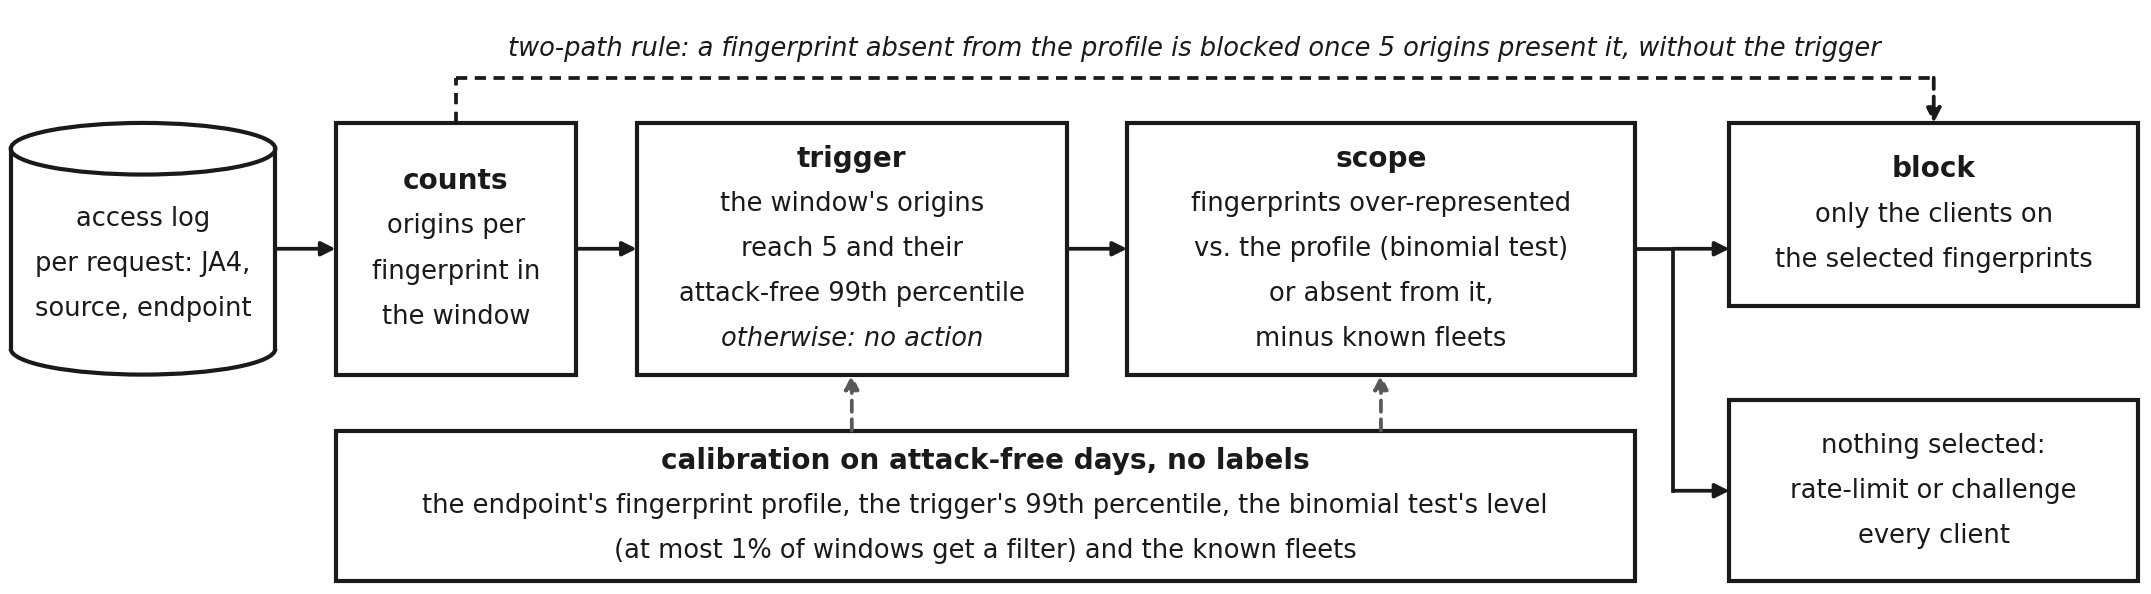
\includegraphics[width=\textwidth]{figures/fig1_scoping.png}
\caption{Per endpoint and five-minute window, the primary configuration blocks clients on selected fingerprints after the trigger fires, or rate-limits or challenges every client if none are selected. The dashed path applies novelty filtering without the trigger (two-path rule, post hoc).}
\label{fig:pipeline}
\end{figure*}


%\textit{Scoping a mitigation.}
Aggregate-based defenses group traffic by packet-header fields and throttle each group~\cite{mahajan2002pushback,alcoz2022accturbo}. Blackholing drops all traffic to attacked destinations, and finer header-based rules narrow what it drops~\cite{dietzel2018stellar}. Source-based filtering selects prefixes under a filter budget, balancing attack coverage against legitimate traffic~\cite{soldo2012filtering}. These approaches show how filter granularity affects collateral, but none selects clients by TLS fingerprint.

Selection against a baseline has a longer history (Table~\ref{tab:related}). Anomaly extraction isolates feature values over-represented in abnormal traffic~\cite{silveira2010urca,brauckhoff2009extraction}, and feature distributions~\cite{lakhina2005mining}, change detection~\cite{krishnamurthy2003sketch} and signature generation~\cite{li2006hamsa} also compare traffic with a baseline. The closest mitigation, PacketScore~\cite{kim2006packetscore}, scores each packet against a nominal profile and drops the lowest scores under overload. Commercial edge systems push signature rules generated in real time~\cite{yoachimik2021dosd} without publishing how they choose them or what they cost legitimate users. We calibrate the profile comparison for TLS fingerprints under correlated legitimate clients and measure its cost on production traffic.
%Our calibrated test asks the same question of TLS fingerprints, relative to each endpoint's normal traffic.

%\textit{Layer-7 detection.}
Application-layer DDoS detectors, from traffic profiles and session features~\cite{tripathi2021application} to PCA~\cite{fernandes2015autonomous,bharathi2012pca}, learned models~\cite{kemp2023approach} and knowledge-graph detectors such as KLAGE~\cite{belcastro2025klage}, stop at a verdict that names no filter. Request patterns separate flash crowds from attacks~\cite{xie2009monitoring}. Defenses that act on every client instead, with CAPTCHAs~\cite{kandula2005botz} or a payment in bandwidth~\cite{walfish2006speakup}, burden all legitimate clients, as the fallback in Fig.~\ref{fig:pipeline} does.

%\textit{Knowledge graphs and fingerprints.}
Passive TLS fingerprinting identifies client software from its handshake~\cite{husak2016https}, and measurements at scale map fingerprints to libraries and applications~\cite{anderson2019tls,kotzias2018coming,razaghpanah2017studying}, so a fingerprint shared by one library's applications both enables filtering and creates collateral risk. A technical report mitigates HTTPS floods by JA3, JA4's predecessor, in a security operations center and reports evasion by extension reordering~\cite{kobayashi2024ja3}. Evaluations of anti-bot services and browser fingerprinting measure how bots evade detection~\cite{aminazad2020webrunner,vastel2020fpcrawlers}.

Table~\ref{tab:related} summarizes these lines of work. None of them measures what a fingerprint filter costs legitimate clients on production traffic, which is the gap this work addresses.

%% ====================================================================
%% ===== end sections/relatedwork.tex =====

%% ===== begin sections/main.tex =====
%% ====================================================================
\section{Calibrated Fingerprint Scoping}
\label{sec:approach}

We compare fingerprints observed during an alarm with an endpoint-specific baseline, selecting those that are either over-represented or absent from the profile. Figure~\ref{fig:pipeline} illustrates the filtering pipeline, including its volume trigger and endpoint-specific calibration.

\subsection{Threat Model}
\label{sec:threat}

The defender operates the targeted application and terminates its TLS.
For each request, it records the TLS \textit{ClientHello},
source address with prefix and ASN, endpoint,
arrival time, and any application identity.
From the \textit{ClientHello}, it computes a JA4
fingerprint~\cite{althouse2023ja4}, which summarizes
the TLS version, cipher suites, extensions and ALPN. 
The defender sees neither the botnet's control channel nor which
sources are coordinated, but can profile traffic outside attacks.

The attacker controls $K$ compromised devices and
may make each session statistically indistinguishable
from a legitimate one, as our evaluation assumes. Each session holds a connection and worker as
legitimate traffic does, so no per-session rate rises. We assume a bot keeps the fingerprint of its TLS stack (its library). How many stacks a botnet spans is unmeasured. Bots that carry their own library put a botnet on one stack, which is easy to select, whereas bots that use their hosts' libraries could spread it over the many device models botnets span~\cite{antonakakis2017mirai}. We therefore take 25 stacks as an intermediate case and assume them new or rare at the endpoint, whose traffic concentrates on a few fingerprints (Section~\ref{sec:method}). The operator's endpoints have no DDoS labels: their web application firewall (WAF) marks routine blocks. These labels do not support this premise, since the origins our filters select were WAF-blocked less often than a random pick (Appendix~\ref{app:window}). The edge's labels in two real attacks do (Section~\ref{sec:real}).
Imitating a browser's \textit{ClientHello} takes a full
browser or an impersonation library that tracks browser releases~\cite{frolov2019tls}. Such bots fall outside our threat model, and Section~\ref{sec:results} tests them as a boundary case.

\subsection{The Trigger}
\label{sec:rule}

For each endpoint $e$ and five-minute window (Fig.~\ref{fig:pipeline}), let $S$ be the sessions to $e$ and $n$ their distinct \textit{origins}, each an address--fingerprint pair. An origin here is unrelated to a CDN's origin server.
On production traffic, the \textbf{origin trigger} fires when the window's count of origins is at least $k_{\min}=5$ and reaches its 99th percentile on attack-free windows. That count also includes plain-HTTP clients, which $n$ omits, because the trigger measures load while the scope needs fingerprints.



\subsection{The Scope and Its Calibration}
\label{sec:evidence}

The scope determines which clients a mitigation would
affect. Selecting the alarm's most common (modal)
fingerprint is unreliable because it may belong to
legitimate users: with the measured $38.4\%$ share of the
most common fingerprint (Section~\ref{sec:method}) and a
campaign as large as legitimate traffic, the modal fingerprint
belongs to the attack only while the botnet spans fewer than
three stacks (Appendix~\ref{app:window}). With more stacks,
the modal filter blocks legitimate clients and no attackers.

We therefore compare the alarm's origins with a \textbf{profile} of
the endpoint's normal traffic.
Let $b(f)$ be the share of fingerprint $f$ among the
profile's $N$ pooled origins, plus $1/N$
so that no background is zero. Let
$c(f)$ count the alarm's origins presenting $f$, and
$n=\sum_f c(f)$. The \textbf{binomial enrichment test}
selects every $f$ that is both enriched, $c(f)/n \geq \rho
b(f)$ with $\rho=3$, and unlikely at level $\lambda_e$,
$\Pr[X\geq c(f)]<\lambda_e/|F|$ for
$X\sim\mathrm{Bin}(n,b(f))$. The Bonferroni divisor
$|F|$ counts fingerprints in the profile and alarm.
The test selects a \textit{set} of fingerprints, covering a botnet spread over several stacks.

The \textbf{$z$-score} compares $c(f)$ with its
binomial background. The uncalibrated \textbf{novelty rule} selects fingerprints absent from the profile (\textit{unseen}) once $k_{\min}$ origins present them. Its \textbf{union} with the test adds the new stacks that the test misses.

On generated traffic, each origin carries one session
and $\lambda_e=0.01$. Production traffic differs, however: legitimate client \textit{fleets} can become active together, violating the binomial independence assumption, and at level $0.01$ the test would select a filter in $26.9\%$ of attack-free windows.
We therefore calibrate $\lambda_e$ per endpoint as the
largest value up to $0.01$ at which the scope selects a
filter in at most $1\%$ of attack-free
calibration windows, our \textit{false-alarm budget}.
At levels such as $10^{-60}$, the binomial tail is no longer
a reliable probability and serves as a score calibrated on
observed traffic.
The $z$-score threshold, the 99th percentile of each
window's largest score and never below 3, meets the same
budget. Both scopes satisfy
the budget on calibration windows by construction.


The profile requires no attack labels, but must exclude
attack episodes. Otherwise, a campaign spanning the
profile would no longer appear enriched. Conversely, attackers on a common legitimate fingerprint may not enrich it enough to be selected, and the scope then cannot tell them from normal clients.

\subsection{The Calibration Floor}
\label{sec:floor}

Calibration limits false alarms but also raises the minimum
attack size needed for selection. We call this the
\textbf{calibration floor}: the botnet size from which the
scope selects a typical stack.
For a stack with $c$ attackers among $n$ origins, the test
requires $c/n\geq\rho b(f)$ and
$\Pr[X\geq c]<\lambda_e/|F|$.
The floor is the smallest $A$ for which a stack of $0.9A/M$
attackers passes both in a window of $n_0+A$ origins, where
$n_0$ is the
median calibration window. Stricter levels raise
this floor.

In the union, the novelty rule selects a stack absent from the
profile once it has $k_{\min}$ origins, requiring $\lceil
k_{\min}M/0.9\rceil$ attackers at any level, 139 for $M=25$.
Shared fingerprints need the calibrated test, and there
$\rho$ sets an \textit{enrichment limit}: a stack's expected
share stays below $0.9/M$, so a fingerprint whose background
share exceeds $0.9/(\rho M)$, $1.2\%$ for $M=25$ and
$\rho=3$, is not expected to be selected.

We evaluate two ways to lower the floor.
First, \textit{known fleets} are fingerprints selected
at level $0.01$ in at least $5\%$ of calibration
windows. Exempting them from the scope and calibration acts as an allow-list on the busiest
endpoint and the API. These fingerprints carry up to about $7\%$ of their profiles, and the scope never blocks
attackers using them. Second, a \textbf{beta-binomial background} tests each profile fingerprint's count against a beta-binomial with the same mean and a within-window correlation fitted on calibration windows (Appendix~\ref{app:window}).



%% ====================================================================
%% ===== end sections/main.tex =====

%% ===== begin sections/eval-methodology.tex =====
\section{Evaluation Methodology}
\label{sec:method}

We use three traffic sources. A generator calibrated on benign CICIDS2017 sessions~\cite{sharafaldin2018cicids} and CDN-measured JA4 fingerprints runs controlled campaigns. Twenty-three days of four CDN endpoints measure false alarms and, with injected botnets, coverage, and a customer's site gives two real attacks.

\subsection{Scenarios and Datasets}

%\textbf{Controlled evaluation: calibrated synthetic traffic.}
A generator produces distributed Slow HTTP DoS campaigns against a single endpoint with known ground truth. Its main parameter is $K$, the number of attacker-controlled devices. We evaluate $K=50$, a small botnet whose sources stay below their rate limits, and $K=1000$, spread across hundreds of /24 prefixes, so that no per-session feature separates bots from clients. Legitimate fingerprint popularity follows a Zipf distribution with exponent $\alpha$, reflecting the concentration of real client~populations.

To calibrate this distribution, we analyze $6.33$M TLS requests recorded at a production edge point of presence of Azion Technologies\footnote{Measured on August 22, 2026, from an existing platform access log. The extract contains only client-software fingerprints and their frequencies, with no addresses, hosts, URIs, headers, or locale.}. Its 495 distinct fingerprints are highly concentrated: the most common accounts for $38.4\%$ of requests, and the top ten for $93.8\%$. The most common fingerprint's share is consistent with $\alpha=1.5$, while the top ten more closely match $\alpha=2.0$, so we use $\alpha=1.5$ by default.

No published measurements establish how botnets are distributed across TLS stacks, so we vary this distribution. We assign $90\%$ of attacker devices uniformly at random across $M$ stacks, a difficult case for selecting a stack at a given $M$, and give the remaining $10\%$ unique fingerprints. We set $M=25$ by default. In \textit{shared} mode, attackers use fingerprints from the profile's tail, rare ones that legitimate clients also present. In \textit{adversarial} mode, they use the most common legitimate fingerprints, modeling bots that imitate popular browsers.

Legitimate request counts and durations are sampled from benign CICIDS2017 sessions.  In \textit{stealth} mode, attacker sessions follow the same distributions, so only their fingerprints set them apart. Attackers start within the first 30~s, accounting for a median $34$--$45\%$ of origins in attack windows and, at $K=1000$, $50\%$ of the alarm's \textit{cluster}. A cluster chains sessions to one endpoint starting at most 300~s apart.

%\textbf{Production traffic.}
On production traffic, we use eight initial days from four Azion service endpoints: real-user monitoring beacons (E1), a web console (E2), an API (E3), and single sign-on (E4). Their median windows hold about 3,000, 62, 41 and 20 origins. Of 12 exported endpoints, we select the four that use TLS and provide at least 50 calibration windows, with a median of at least $k_{\min}$ origins per window. The exports contain distinct origins and connections per fingerprint and window, and same-/24 pairs. The scope is evaluated offline behind the operator's WAF, so profiles and floors describe the clients it admits. Pre-injection test windows count as \textit{clean}, so a real attack there counts as a false alarm.

We assume calibration days are attack-free. An attack there would lower the test level and raise the trigger threshold, so false alarms would fall, but its fingerprints would enter the profile and stop looking enriched.

Each of the last five initial days, the \textit{development days}, is evaluated using profiles, thresholds, and levels derived from earlier days, and the design choices of Section~\ref{sec:configs} were made on them. We inject generated botnets into each window, varying the number of attackers from 25 to 1,000 or from $0.1\times$ the median window size, about 300 attackers on E1, to $1\times$. We assign $90\%$ of attackers uniformly at random to 25 stacks and the remainder to unique fingerprints that the scope cannot select, limiting the maximum blockable fraction to approximately $90\%$. Attacker fingerprints are either absent from the observed traffic (\textit{new}), drawn from the profile's tail beyond its ten most common fingerprints (\textit{shared}), or selected from the endpoint's 25 most common fingerprints (\textit{adversarial}). We also simulate flash crowds by adding 100 or 1,000 of the day's clients to a single window. A ninth day (\textit{held-out day}) and 14 later days (\textit{prospective period}) are evaluated as fixed in advance. A fifth endpoint (E5), a customer's e-commerce site, adds eight later days, the last with two real attacks, analyzed post hoc in Section~\ref{sec:real}.

\subsection{Baselines, Configurations and Metrics}
\label{sec:configs}

On generated traffic, we compare four scopes applied to the alarm's cluster: the modal fingerprint, the novelty rule, the $z$-score ($z>3$), and the binomial test. On production traffic, we evaluate the configurations in Table~\ref{tab:configs}, estimating thresholds, levels and known fleets on attack-free days. \textit{In sample}, each calibration day is assessed against a profile that includes its own traffic, making its fleets appear less enriched. In \textit{cross-fitting}, introduced post hoc, it is assessed against a profile built from the other days, as for a development day.

\begin{table}[!ht]
\centering
\caption{The calibrated configurations on production traffic}
\label{tab:configs}
\scriptsize
\setlength{\tabcolsep}{3pt}
\begin{tabular}{@{}llll@{}}
\toprule
\textbf{Configuration} & \textbf{Trigger} & \textbf{Scope} & \textbf{Fleets} \\
\midrule
\multicolumn{4}{@{}l}{\textit{Fixed on the development days: the primary (test 1), then two references}} \\
Primary                       & origins        & binomial $\cup$ novelty    & exempt \\
$z$-score                     & origins        & $z >$ its p99              & no \\
Base rule                     & $\Omega$       & binomial                   & no \\
\rowcolor[gray]{0.90}
\multicolumn{4}{@{}l}{\textit{Pre-registered after the held-out day: the novelty rule and two arms (tests 2 and 3)}} \\
\rowcolor[gray]{0.90}
Novelty rule                  & none           & novelty                    & no \\
\rowcolor[gray]{0.90}
Beta-binomial arm$^{\dagger}$ & seasonal       & beta-bin.\ $\cup$ novelty  & no \\
\rowcolor[gray]{0.90}
No-trigger arm, E1 only       & none           & binomial $\cup$ novelty    & exempt \\
\multicolumn{4}{@{}l}{\textit{Post hoc}} \\
Two-path rule                 & none / origins & novelty / binomial         & exempt \\
\bottomrule
\end{tabular}

\vspace{2pt}
\begin{minipage}{\linewidth}\footnotesize The held-out day's protocol fixed only the primary and the base rule. $^{\dagger}$Cross-fitted. $\Omega$: an earlier design, mostly counting volume (Appendix~\ref{app:window}).\end{minipage}
\end{table}

Five choices were made using the development days: counting origins, calibrating $\lambda_e$, choosing the origin trigger, adding the novelty rule to the test, and setting the fleet-share threshold to $5\%$ by its false-alarm count. A $0.5\%$ threshold produced more false alarms, with lower median collateral and higher coverage (Appendix~\ref{app:window}). An initial cross-fitting design, calibrated on one day, was dropped after its results were seen, because one day misses the rare fleet events that set the level. The values $\rho=3$ and $k_{\min}=5$, the triggers' 99th percentile and 25 stacks were fixed on generated traffic before any endpoint's data were seen.


We define \textbf{collateral damage} as the share of a window's legitimate origins that the selected filter blocks, which is its false-positive rate if deployed. An address with two fingerprints counts twice, and an origin-window is an origin in a window. On production traffic, the \textbf{false-alarm rate (FA)} is the share of clean windows where a configuration selects a filter. We evaluate 5,643 eligible windows on the development days and 1,152 on the held-out day, excluding those under $k_{\min}$ origins. Exact 95\% intervals assume independent windows, but false alarms may cluster by day, so we also give daily counts. Tables give the median collateral over false alarms (\textbf{FA coll.}), and the false-alarm rate times the mean collateral is the expected share of origins blocked per clean window.

The tables also report the scope's false-alarm rate when it runs on every window as its own trigger (\textit{No trigger}, or \textit{None} in the Trigger columns), its rate under 1,000-client flash crowds (\textit{Crowds}), and botnet coverage when the attack size equals the median window size or one-tenth of it ($1\times$ and $0.1\times$). Coverage is averaged over all attack windows, including those in which the trigger does not fire. It therefore reflects whether the trigger fires and what the scope selects.
%% ====================================================================
%% ===== end sections/eval-methodology.tex =====

%% ===== begin sections/results.tex =====
\section{Results}
\label{sec:results}

The pre-registered 14-day evaluation makes the coverage--cost trade-off explicit (Table~\ref{tab:overview}). The primary pipeline selected a filter in 31 of 16,103 clean five-minute windows ($0.19\%$), but the median false alarm would have blocked $39\%$ of its window's legitimate origins. Its fallback also challenged or rate-limited $0.6\%$ of clean origin-windows, compared with $0.016\%$ blocked by the filters. A low rate of filter selection therefore describes only part of the exposure.

\begin{table}[!ht]
\centering
\caption{What the policies deliver over the 14-day prospective period}
\label{tab:overview}
\footnotesize
\setlength{\tabcolsep}{2.3pt}
\begin{tabular*}{\columnwidth}{@{\extracolsep{\fill}}lrrrr@{}}
\toprule
\textbf{Policy} & \textbf{Bots} & \textbf{Clean} & \textbf{Legit.} & \textbf{Fallback} \\
\midrule
Primary                  & 2.9  & 0.19 & 39.0 & 0.6 \\
Novelty, no trigger      & 89.6 & 0.00 & n/a  & -- \\
Origin cap (post hoc)    & 57   & 1.5  & 0.7  & -- \\
\bottomrule
\end{tabular*}

\vspace{2pt}
\begin{minipage}{\linewidth}\footnotesize In \%, E1--E4. Bots: E1's $0.1\times$ botnet on new fingerprints ($\approx300$ bots); filters block, the cap challenges. Clean: windows with an action. Legit.: median legitimate-origin share in those windows. Fallback: challenged or rate-limited clean origin-windows. Cap: exploratory; other rows: pre-registered. n/a: no false alarm in E1--E4; --: no fallback.\end{minipage}
\end{table}

For approximately 300 bots on new fingerprints at E1, the busiest endpoint, the primary pipeline blocked $3\%$, versus $90\%$ for novelty filtering without the trigger. The cap, an exploratory comparison on the same period, challenged $57\%$ and acted more often on clean windows but affected fewer origins when it did. These are distinct actions, so the table compares exposure rather than an interchangeable measure of harm. Novelty filtering also needs validation per site: at the customer site E5 it raised false alarms in $8.9\%$ of clean windows, with median collateral of $0.24\%$ per false alarm (Section~\ref{sec:real}).

\subsection{What the Scope Can Select}
\label{sec:symbolic-detector}
\label{sec:fleetfloor}
\label{sec:production}
\label{sec:collateral}
\label{sec:ablation}



Generated traffic isolates selection under a constructed best case: its new stacks never appear in legitimate traffic. The following development-day measurements explain the mechanisms behind the prospective results; they shaped the design and are not independent confirmation.

On generated traffic (Appendix~\ref{app:window}, Table~\ref{tab:symbolic}), the modal fingerprint belongs to legitimate clients from five stacks onward, as Section~\ref{sec:evidence} predicts, so it covers no attackers and blocks its $39.0\%$ share of legitimate traffic. In contrast, the profile-relative scopes cover about $90\%$ of attackers on up to 25 new stacks, the cap that one-off fingerprints set, with no observed collateral except the novelty rule's mean $0.03\%$. At 100 stacks, the novelty rule still covers $88.1\%$ at that collateral, whereas the test, with too few attackers per stack, covers $38.6\%$. Shared and adversarial stacks also bring collateral: on adversarial ones, the test covers $30.4\%$ of attackers while blocking $3.78\%$ of legitimate traffic (Table~\ref{tab:symbolic}). A volume trigger alone can also fire on flash crowds~\cite{jung2002flash}, which the test suppresses for generated crowds but not for all production crowds.

The strict calibration that keeps false alarms rare also raises the floor. Legitimate client fleets drive $\lambda_e$ to levels between $10^{-4}$ and $10^{-73}$ (\cf Table~\ref{tab:floor}); exempting known fleets raises the busiest endpoint's from $10^{-60}$ to about $10^{-21}$. For a botnet on 25 new stacks, the novelty rule sets the floor at 139 attackers per window on E1--E3, when an average stack reaches $k_{\min}$; on E4 the test selects stacks first, from 84.

\begin{table}[!h]
\centering
\caption{Calibration floor, in attackers per window}
\label{tab:floor}
\scriptsize
\setlength{\tabcolsep}{2.2pt}
\begin{tabular}{@{}lccccccc@{}}
\toprule
 & & \multicolumn{2}{c}{$\lambda_e$} & \multicolumn{2}{c}{\textbf{Primary}} & \multicolumn{2}{c}{\textbf{Beta-binomial arm}$^{*}$} \\
\cmidrule(lr){3-4}\cmidrule(lr){5-6}\cmidrule(l){7-8}
\textbf{Endpoint} & $n_0$ & bin. & beta$^{*}$ & new & shared & new & shared \\
\midrule
E1, beacons     & 2,983  & $10^{-21}$ & $10^{-4}$ & 139/139 & 254/286 & 85/139 & 86/167 \\
E2, web console & 62      & $10^{-73}$ & $10^{-2}$ & 139/139 & 1090/1041 & 56/114 & 84/168 \\
E3, API         & 41      & $10^{-11}$ & $10^{-2}$ & 139/139 & 168/227 & 56/114 & 56/140 \\
E4, sign-on     & 20      & $10^{-4}$ & $10^{-2}$ & 84/84 & 84/114 & 56/56 & 84/84 \\
\bottomrule
\end{tabular}

\vspace{2pt}
\begin{minipage}{\linewidth}\footnotesize Floors: botnet size from which the scope alone selects a typical stack of a 25-stack botnet, in sample / cross-fitted, development-day medians. Table~\ref{tab:block} uses the primary in sample and the arm cross-fitted. $n_0$: median origins per window. $\lambda_e$ in sample. $^{*}$Added after the held-out day, as was cross-fitting.\end{minipage}
\end{table}

Shared fingerprints depend instead on the calibrated level. On the busiest endpoint, a 25-stack botnet on them needs 254 attackers, $8.5\%$ of the median window, and on the smaller endpoints 4 to 18 median windows (Table~\ref{tab:floor}). The floor rises with the number of stacks and with fingerprint popularity (Appendix~\ref{app:window}), but it is not a hard threshold: a binomial model of the injection predicts $43.1\%$ coverage without the trigger for 100 attackers on new stacks at E1, close to the measured $43.2\%$ (Fig.~\ref{fig:stops}).

Botnets on an endpoint's most common fingerprints fall outside our threat model, and the enrichment limit largely excludes them: the configuration blocks $7.0\%$ of 100 such attackers and $23.8\%$ of 1,000, none on the two largest endpoints.

\subsection{Coverage Lost to the Trigger}
\label{sec:trigger}

\begin{figure}[t]
\centering
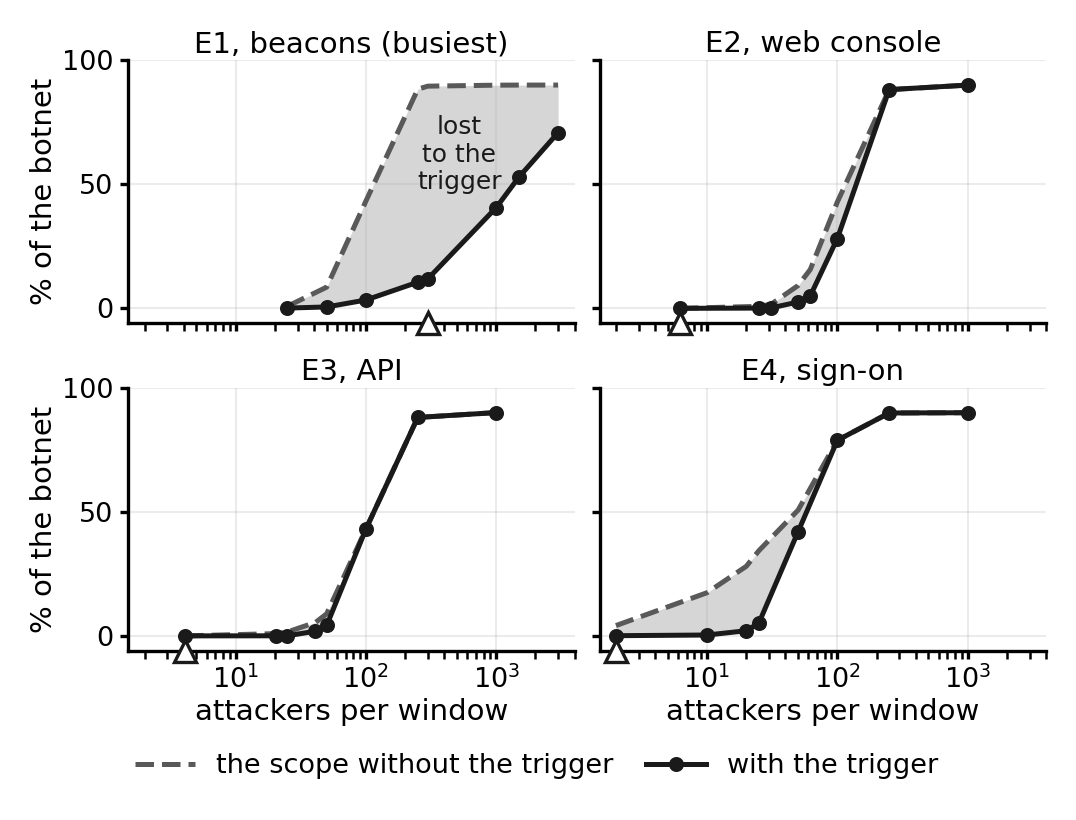
\includegraphics[width=\columnwidth]{figures/fig6_stops.png}
\caption{Coverage of 25-stack botnets on new fingerprints during development days: primary configuration (solid) and scope without the trigger (dashed, post hoc). Shading shows coverage lost to the trigger; triangles mark $0.1\times$ the median window. One-off fingerprints cap coverage near $90\%$. On E1--E3, the dashed curve also represents the two-path rule's novelty path.}
\label{fig:stops}
\end{figure}

On the development days, the scope alone selected a filter in $2.2\%$ of clean windows. Requiring the volume trigger reduced joint false alarms to $0.1\%$ (5/5,643), which motivated the safeguard; the prospective results show how much coverage it can lose.

A selected fingerprint blocks attackers only when the trigger also fires (\cf Figure~\ref{fig:stops}). On the busiest endpoint, the trigger fires in just $6$--$13\%$ of windows for botnets from 25 attackers to $0.1\times$. The primary configuration therefore blocks only $3.4\%$ of a 100-attacker botnet and $11.8\%$ of a $0.1\times$ botnet, whereas without the trigger the scope would cover $43.2\%$ and $89.6\%$. On the smaller endpoints, in contrast, 100 attackers are 1.6--5 median windows and fire the trigger in $66$--$100\%$ of windows, so the floor is the main limit there. On these smaller endpoints, a $1\times$ botnet fires it in only $14$--$33\%$ of windows.

%\textbf{Other triggers.}
Two alternatives added after the held-out day show what the trigger costs (Table~\ref{tab:triggers}). A \textit{seasonal trigger}, which divides distinct origins by the same hour's calibration median and fires past the 99th percentile of that ratio, raises coverage of that botnet on new stacks only from $12\%$ to $20\%$. With the binomial test, it also exceeds the budget on one smaller endpoint ($2.64\%$). Without a trigger, the scope covers about $90\%$ of it on every day, and the novelty rule matches the test with fewer false alarms and crowd firings.

\subsection{Reference Variants and Post Hoc Checks}
\label{sec:posthoc}
\label{sec:boundary}


\textit{Evaluation protocol.} On the held-out day, the primary configuration produces two false alarms in 1,152 clean windows, consistent with the development-day rate ($P = 0.27$). We published the protocol of the prospective period (public commit 05ccc0e) before exporting or reading any of its days. It fixed Table~\ref{tab:configs}'s six configurations and three tests: whether the primary's false-alarm rate matches the development days'; whether the novelty rule and two arms stay within budget per endpoint; and which arm within budget beats the novelty rule's coverage by at least one point on new or shared stacks. An addendum published before any result was computed (ad7c03b) moved the third test from a $0.1\times$ botnet, 2 to 7 attackers on E2--E4, to 100 attackers; both versions prefer the same arm (Appendix~\ref{app:window}).

\textit{Pre-registered comparisons.} The primary's prospective false-alarm rate was about twice the development-day rate, but below the $1\%$ budget (95\% interval $0.12$--$0.27\%$, resampling endpoint-days). The first test treats the development-day rate, estimated from five false alarms, as known and finds the rates inconsistent ($P<10^{-4}$); a post hoc Fisher test accounting for that uncertainty is inconclusive ($P=0.07$). In the second test, the novelty rule and beta-binomial arm stay within budget on every endpoint, while the no-trigger arm on E1 does not ($1.56\%$). The third prefers the beta-binomial on every endpoint, though its false alarms blocked a median $65.7\%$ of their windows' origins.

The calibrated $z$-score, a pre-registered reference, beat the primary configuration prospectively on false alarms, on 100 new-stack attackers and on 1,000-client flash crowds (Table~\ref{tab:block}). On the development days, however, it raised four times as many false alarms (20 versus 5) and exceeded the budget on the web console ($1.1\%$). Those false alarms blocked a median $10.8\%$ of their windows' origins, versus $32.9\%$. The two configurations thus trade places between periods.

\begin{table}[!ht]
\centering
\caption{Prospective results for reference configurations and variants}
\label{tab:block}
\scriptsize
\setlength{\tabcolsep}{1.8pt}
\begin{tabular}{@{}lccccccccc@{}}
\toprule
 & \multicolumn{3}{c}{\textbf{False alarms}} & & & \multicolumn{2}{c}{\textbf{E1, $0.1\times$}} & \multicolumn{2}{c}{\textbf{100 attackers}} \\
\cmidrule(lr){2-4}\cmidrule(lr){7-8}\cmidrule(lr){9-10}
\textbf{Configuration} & all & E1 & E2--E4 & \textbf{FA coll.} & \textbf{Crowds} & New & Shared & New & Shared \\
\midrule
\multicolumn{10}{@{}l}{\textit{Fixed on the development days: the primary (test 1), then two references}} \\
Primary                       & 0.19 & 0.00 & 0.42          & 39.0 & 18.8 & 2.9  & 2.4  & 36.8 & 22.1 \\
$z$-score                     & 0.12 & 0.00 & 0.30          & 40.1 & 3.0  & 3.0  & 2.6  & 56.2 & 26.9 \\
Base rule                     & 0.26 & 0.00 & 0.69          & 46.6 & 16.8 & 0.0  & 0.0  & 29.4 & 22.0 \\
\rowcolor[gray]{0.90}
\multicolumn{10}{@{}l}{\textit{Pre-registered after the held-out day: the novelty rule and two arms (tests 2 and 3)}} \\
\rowcolor[gray]{0.90}
Novelty rule                  & 0.00 & 0.00 & 0.00          & n/a  & 2.7  & 89.6 & 0.0  & 43.2 & 0.0 \\
\rowcolor[gray]{0.90}
Beta-binomial arm$^{\dagger}$ & 0.12 & 0.35 & 0.05          & 65.7 & 33.5 & 11.8 & 11.4 & 61.0 & 39.7 \\
\rowcolor[gray]{0.90}
No-trigger arm$^{a}$          & --   & \textbf{1.56} & --    & --   & --   & 89.6 & 67.7 & --   & -- \\
\multicolumn{10}{@{}l}{\textit{Post hoc: the two-path rule, the novelty and primary rows combined}} \\
Two-path rule                 & 0.19 & 0.00 & 0.42          & 39.0 & 18.8 & 89.6 & 2.4  & 52.1 & 22.1 \\
\bottomrule
\end{tabular}

\vspace{2pt}
\begin{minipage}{\linewidth}\footnotesize In \%, 16,103 clean windows, calibrated on all earlier days, in sample except $^{\dagger}$cross-fitted. E2--E4: their highest. FA coll. (median per false alarm), Crowds, 100 attackers: pooled. E1, $0.1\times$: about 300 attackers. Bold: above the $1\%$ budget; n/a: no false alarm; --: not computed. $^{a}$E1 only: FA coll. 4.3, Crowds 1.2, 100 attackers 43.4 and 4.5.\end{minipage}
\end{table}


The beta-binomial arm, behind the seasonal trigger, covers $61\%$ of 100 new-stack attackers, versus $43\%$ for the novelty rule, and $40\%$ on shared stacks, which the novelty rule cannot select (Table~\ref{tab:block}). On the busiest endpoint, however, it adds $11.4\%$ of the $0.1\times$ botnet on shared stacks but covers only $11.8\%$ on new stacks, versus $89.6\%$ for the novelty rule.

\textit{Post hoc comparisons.} The two-path rule combines novelty filtering without the trigger with calibrated selection of rare shared fingerprints behind it. It was fixed before E5 but remains an exploratory hypothesis. It raised false alarms in $0.28\%$, $0.26\%$ and $0.19\%$ of clean windows across the development, held-out and prospective periods, respectively; on the held-out console its rate exceeded budget ($1.04\%$). At E5, the beta-binomial arm stopped $10\%$ and $0\%$ of attackers, adding little to novelty's $9\%$ in the first attack.

The stages' false alarms were dependent: prospectively they coincided in 31 clean windows, where endpoint-wise independence predicts 2.87. The excess persisted after stratification by time or window size; the supporting tests, weekday analysis and multiplicity correction are in Appendix~\ref{app:window}.

In a \textit{one-hour replay}, each false alarm's filter acts from the next window for 12 windows. Across the same 31 alarms, the median of the per-alarm mean collateral over those windows was $0.36\%$, compared with $39\%$ in the selecting windows. Overall, filters would have blocked $0.012\%$ of clean origin-windows. E1 holds $95\%$ of origin-windows and had no false alarm, so on E2--E4 they blocked $0.03$--$0.58\%$ per endpoint, while the fallback challenged or rate-limited $0.65$--$7.1\%$.

A history baseline tests each fingerprint's count against its own calibration history. Under the same trigger and budget, the binomial test alone, without the novelty rule or known fleets, raised fewer false alarms (31 versus 78 prospectively, 6 versus 52 on the development days), though prospectively only because of E4 (4 versus 54). It also stopped more of 100 attackers ($29\%$ and $22\%$ on new and shared stacks, versus $12\%$) and fired less in flash crowds ($17\%$ versus $75\%$).

The per-fingerprint origin cap of Table~\ref{tab:overview} (Appendix~\ref{app:window}) covers $1.9\%$ of E1's $0.1\times$ botnet behind the trigger and $14\%$ of 100 attackers pooled, whose stacks rarely exceed it.

\subsection{Two Real Attacks}
\label{sec:real}

\begin{table}[t]
\centering
\caption{Two real attacks at a customer's site (E5), post hoc}
\label{tab:real}
\scriptsize
\setlength{\tabcolsep}{2.0pt}
\begin{tabular}{@{}lccccccccc@{}}
\toprule
 & \multicolumn{4}{c}{\textbf{Attack 1}} & \multicolumn{4}{c}{\textbf{Attack 2}} & \\
\cmidrule(lr){2-5}\cmidrule(lr){6-9}
\textbf{Filter} & Req. & Att. & Leg. & Leg.$^{e}$ & Req. & Att. & Leg. & Leg.$^{e}$ & \textbf{FA} \\
\midrule
\multicolumn{10}{@{}l}{\textit{Primary configuration}} \\
Selecting window    & 47.2 & 32.7 & 0.05 & 2.58 & 48.1 & 47.5 & 0.09 & 0.14 & 0.43 \\
A window late       & 36.5 & 30.4 & 0.02 & 1.61 & 35.7 & 27.5 & 0.05 & 0.07 & \\
Late, kept to end   & 36.5 & 31.3 & 0.02 & 2.29 & 43.0 & 38.0 & 0.07 & 0.09 & \\
\rowcolor[gray]{0.90}
\multicolumn{10}{@{}l}{\textit{Other configurations, in the selecting window}} \\
\rowcolor[gray]{0.90}
$z$-score                         & & 33.2 & 0.05 & & & 48.8 & 0.15 & & 0.43 \\
\rowcolor[gray]{0.90}
Novelty rule                      & & 8.8  & 0.00 & & & 0.0  & 0.00 & & \textbf{8.94} \\
\rowcolor[gray]{0.90}
Beta-binomial arm                 & & 10.4 & 0.00 & & & 0.0  & 0.00 & & 0.52 \\
\rowcolor[gray]{0.90}
Two-path rule, post hoc & 47.2 & 32.7 & 0.05 & 2.58 & 48.1 & 47.5 & 0.09 & 0.14 & \textbf{8.94} \\
\bottomrule
\end{tabular}

\vspace{2pt}
\begin{minipage}{\linewidth}\footnotesize In \%, summed over each attack's windows. Req.: requests on the selected fingerprints. Att., Leg.: attackers' and legitimate origins blocked, Leg.$^{e}$ when only edge-blocked addresses count as attackers. FA: false alarms in E5's 1,152 windows of four attack-free days, bold above the $1\%$ budget.\end{minipage}
\end{table}

E5 is a customer's site with a median window of about 3,700 origins. Unlike in our threat model, the bots exceeded the edge's rate limits and mostly presented browser-like fingerprints. A window late, the primary configuration's filters would have removed $36\%$ of each attack's requests while blocking under $0.1\%$ of legitimate origins. Fingerprint rotation inflated the trigger's count: with each address the edge blocked counted once per window, at most three of the nine windows where it fired would have reached the same threshold. We fixed the two-path rule and every parameter before seeing E5's traffic. Its seven attack-free days set the attack day's profile, trigger threshold, level and known fleets, and each of the last four, profiled on the days before it, measures false alarms. On the eighth day, two attacks, the first of 35 minutes and the second in two waves of 15, raised its requests up to nearly 2,000-fold over the hour before, and the edge blocked them.  Since both stages count origins whatever their rates, the same bots below those limits would have fired the trigger and been selected, if each address still presented the same fingerprints in each window. Their harm to a service is untested.

With the operator's authorization, we analyzed only aggregate exports of E5's logs and report no address, host, network or date that identifies the customer. We label as attackers the origins the edge blocked (HTTP 444 or 429) or that asked only for the root page, and as legitimate those never blocked that asked for other pages. We chose these labels, and the share of requests as a metric, after seeing the attacks. One botnet of about 600 to 2,600 addresses per full window ran both attacks, rotating three browser-like fingerprints: the site's most common Chrome fingerprint, $11\%$ of its profile, and two rare there ($0.003\%$ and $0.16\%$). Its requests split about evenly between the common fingerprint and the two rare ones, so filters that spare the common one can remove about half of them at most. In the first attack, a second botnet, about 4,000 addresses on a library new to the site, joined for 10 minutes.

The origin trigger fired in nine of the 13 attack windows, missing the partial ones at either end.  Behind the trigger, the binomial test selected both rare fingerprints, each carrying 549 to 1,706 attackers per window, and the novelty rule caught the new library. E5's floor is high: a 25-stack botnet on shared stacks needs 2,307 attackers per window, $62\%$ of the median window. Table~\ref{tab:real} gives what these filters would have stopped in the selecting window, a window late, and a window late but kept to the attack's end, known only in hindsight. The first attack's origin share is lower than its request share because $46\%$ of its attackers' origins were on fingerprints other than the two botnets' four, which sent under $1\%$ of its requests. Under the edge label, the selecting window's filters block up to $2.6\%$ of legitimate origins, since up to 524 unblocked addresses per window that asked only for the root page count as legitimate.

Rotation did not hide the rare fingerprints. Almost every attacking address also presented the common one, so few addresses were blocked outright. In the second attack's full windows, each address the edge blocked presented 2.6 to 2.9 fingerprints and at least $80\%$ of them used a rare one. Blocking those addresses would therefore also have reached bots on the common fingerprint, at a cost to users who share them that we did not measure. Selecting the common fingerprint would have needed a third of a window's origins, three times its profile share; the bots brought it to at most $25\%$. With every client in the window and no trigger, $96\%$ of the origins the scopes selected on the attack day were blocked by the edge, versus $42\%$ for a random pick, so these labels support the premise there. On attack-free days, where any selection is a false alarm, the edge blocked $0.01\%$ of their selections, versus $0.34\%$ of a random pick's. On those days, however, the novelty rule fired in $8.9\%$ of windows on fingerprints new that day that the edge never blocked (Table~\ref{tab:real}).
%% ===== end sections/results.tex =====

%% ===== begin sections/discussion.tex =====

\section{Discussion and Limitations}
\label{sec:discussion}



%\textbf{Which configuration to recommend.}
These results support endpoint-specific validation rather than a default configuration. A novelty path needs acceptable clean-window activity and per-alarm collateral at the endpoint where it will run; rare shared fingerprints need the calibrated test and enough supporting origins. The two-path rule combines these choices but remains a post hoc hypothesis (Section~\ref{sec:posthoc}).    

%\textbf{What the evidence supports.}
Most of these results come from injected attacks. The generator isolates fingerprint selection under controlled mimicry, but its campaigns, larger than the $0.1\times$ injections, are easier to catch (Appendix~\ref{app:window}). In the prospective period, the primary configuration stops $58\%$, $37\%$ and $5\%$ of 100 attackers spread over 5, 25 and 100 new stacks, as more stacks leave fewer attackers on each. The real attacks on E5 used a new library and, besides a common fingerprint, two rare ones. One site and one botnet cannot show how common either case is. We did not test challenges on selected fingerprints or prefix filters~\cite{soldo2012filtering}. Bots on a common legitimate fingerprint, or on one per device or connection, evade selection, and libraries such as uTLS~\cite{frolov2019tls} ease both. 

\subsection{Operational Risks}

Without the trigger, novelty filtering becomes a standing policy that can block legitimate clients after browser or application updates until their fingerprints enter the profile. New fingerprints reached $k_{\min}$ origins in $0.21\%$ of development windows, one held-out window, and none of the 16,103 prospective windows. With a three-day profile, novelty filtering would have fired in $0.42\%$ of the console's prospective windows (Appendix~\ref{app:window}). Excluding flagged windows from profile updates resists poisoning but prolongs blocking until operator intervention. Conversely, attackers can seed their fingerprints during normal traffic, forcing later detection to rely on the calibrated test and its floor.

Sections~\ref{sec:symbolic-detector} to~\ref{sec:posthoc} score each filter's coverage only in the window that selected it. A deployed filter acts from the next window and persists. At E5 it stopped less than in that window (Section~\ref{sec:real}). Post hoc, we kept each pick for an hour, redrawing bots' fingerprints every window from a fixed daily stack pool (Appendix~\ref{app:window}). Against E1's $0.1\times$ botnet active all day, filters would have stopped $8.4\%$ of its attackers prospectively, versus $2.9\%$, but persistence cannot make up for the trigger: $91\%$ of that botnet's one-hour attacks, from any starting window, met no filter. The $1\%$ budget allows 2.9 false alarms per endpoint per day and leaves out the fallback. The fallback challenges every client, or rate-limits beacons and API calls that cannot solve a CAPTCHA, and fired 6.5 to 33 times as often as the filters raised false alarms. While a filter is active, the rest of the window meets only the edge's rate limits, so bots on a common fingerprint, as at E5, pass unless also challenged. Origins undercount users who share an address behind a proxy or NAT, so a filter on their fingerprint blocks more users than its collateral shows.

%\textbf{What the data cover.}
\subsection{Data Coverage}

The data cover four of one operator's own endpoints, three of them small, over 23 days, too few to calibrate weekly cycles, and one customer's site over eight days. The busiest endpoint's trigger fired in $5.4\%$ of clean development-day windows but $0.27\%$ of the prospective period's. We recalibrated each day on all earlier days but did not model this drift. Whether attacks near the floor exhaust a service is unknown, since the endpoints' spare capacity was not measured. Only the held-out day and the prospective period evaluate the five development-day choices of Section~\ref{sec:configs}.  Encrypted ClientHello (ECH)~\cite{ietf2026ech} does not hide the inner \textit{ClientHello} from a defender that terminates TLS, as assumed here. We did not test flash crowds of a single client type or attackers that manipulate profiles or fleet exemptions.



%% ====================================================================
%% ===== end sections/discussion.tex =====

%% ===== begin sections/conclusion.tex =====
\section{Conclusion and Future Work}
\label{sec:conclusion}

Endpoint-relative fingerprint profiles can single out bots on fingerprints new or rare to an endpoint; safeguards around the scope shape the coverage and cost of deploying them. In the pre-registered evaluation, the volume trigger cut coverage of a 300-bot botnet on new fingerprints at the busiest endpoint from $90\%$ to $3\%$. False alarms occurred in $0.19\%$ of clean windows, yet the median one would have blocked $39\%$ of its window's legitimate clients, and the fallback exposed far more clients than the filters did. In exploratory replays of two previously mitigated attacks, filters applied one window late would have removed $36\%$ of each attack's requests, with at most $1.6\%$ collateral under two attacker labelings. No configuration dominated. An operator should therefore judge a fingerprint filter by three measurements at each endpoint: coverage behind the trigger, damage per false alarm, and fallback exposure. Future work will test, prospectively across sites, risk-aware policies that filter only when an attack's service degradation outweighs that collateral.
%% ===== end sections/conclusion.tex =====



\section*{Acknowledgment}

We thank Azion Technologies (\url{https://www.azion.com/})
for authorizing the measurements and traffic statistics
in this study.

\section*{Use of AI Disclosure}

The authors used AI assistants (Claude, Anthropic; Codex, OpenAI) to draft and revise text and to write code and figures. All content was reviewed and verified by the authors, who take full responsibility for the work. %An audit script checks 217 table values against the saved results.

\section*{Reproducibility}

The implementation is available at \url{https://github.com/Natanael0liveira/tls-fingerprint-ddos} under the MIT license and is intended for Artifact Evaluation.

\bibliographystyle{IEEEtran}
\bibliography{references}

%% ====================================================================
\appendices

\section{The Base Rule and Production Details}
\label{app:window}

The base rule, a reference in both protocols, scores each window by its coordination mass $\Omega(S) = \sum_i w_i\,|E_i(S)|$, where $E_i(S)$ holds the pairs of distinct origins that share a TLS fingerprint ($w_i = 1.0$), the endpoint ($0.6$) or an IPv4 /24 or IPv6 /48 ($0.3$). Its trigger fires when $\Omega(S)$ reaches its 99th percentile on attack-free windows, and the test then selects the scope. The endpoint term gives $91\%$ of $\Omega$ in the default generated campaign, so $\Omega$ mostly measures volume. Its prospective results are in Table~\ref{tab:block}: its coverage and crowd firings equal those of the binomial test alone, while its false alarms differ (42 versus 31). On the held-out day, it raised two false alarms, as the primary configuration did, and stopped $26.3\%$ and $21.5\%$ of 100 attackers on new and shared stacks, versus $38.9\%$ and $21.5\%$.

\textbf{The modal fingerprint.} For a botnet of $A$ attackers spread uniformly over $M$ stacks, about $0.9A/M$ use each stack and the remaining tenth use one-off fingerprints. If the most common legitimate fingerprint holds a share $p_1$ of $n_b$ legitimate origins, the modal fingerprint belongs to the attack only while $0.9A/M > p_1 n_b$. With $p_1 = 38.4\%$ of requests as a proxy for origins and $A = n_b$, this holds only for $M < 2.3$.

\textbf{Scopes on generated traffic.} For a more concentrated population ($\alpha = 2.0$), the modal scope of Table~\ref{tab:symbolic} blocks $61.1\%$ of legitimate traffic. At 100 stacks, pooling 30 attack-free periods restores the test's coverage to $89.6\%$. The novelty rule's collateral reaches at most $0.5\%$ in one seed. 

\begin{table}[!ht]
\centering
\caption{Each scope alone on generated traffic}
\label{tab:symbolic}
\scriptsize
\setlength{\tabcolsep}{1.6pt}
\begin{tabular}{@{}lcccccc@{}}
\toprule
 & \multicolumn{3}{c}{\textbf{Binomial test}} & \multicolumn{3}{c}{\textbf{Other scopes}} \\
\cmidrule(lr){2-4}\cmidrule(l){5-7}
\textbf{Scenario} & \textbf{Recall} & \textbf{Att.\ coll.} & \textbf{$F_1$} & \textbf{Modal} & \textbf{$z$-score} & \textbf{Novelty} \\
\midrule
$M{=}1$               & 89.8\% & 0.00\% & 0.946 & 89.8\% & 89.8\% & 89.8\% \\
$M{=}5$               & 90.0\% & 0.00\% & 0.948 & 0.0\% & 90.0\% & 90.0\% \\
$M{=}25$              & 90.3\% & 0.00\% & 0.949 & 0.0\% & 90.3\% & 90.3\% \\
$M{=}100$             & 38.6\% & 0.00\% & 0.556 & 0.0\% & 80.4\% & 88.1\% \\
$M{=}25$, shared      & 85.4\% & 2.23\% & 0.910 & 0.0\% & 89.9\% & 0.0\% \\
$M{=}25$, adversarial & 30.4\% & 3.78\% & 0.452 & 3.6\% & 57.3\% & 0.0\% \\
\bottomrule
\end{tabular}

\vspace{2pt}
\begin{minipage}{\linewidth}\footnotesize Recall of each scope alone, capped near $90\%$ since each bot has a one-off fingerprint with probability $0.1$, and the test's collateral in attack windows (Att.\ coll.), $K = 1000$ attackers on $M$ stacks, 15 seeds. Others' collateral: modal $39.0\%$ from $M{=}5$, $z$-score $3.37\%$ (shared) and $11.3\%$ (adversarial).\end{minipage}
\end{table}

\textbf{Triggers on generated traffic.} Over 30 generated runs, the origin trigger fires in $82.2\%$ and $85.7\%$ of attack windows at $K = 1000$ and $K = 50$, and with the test on no clean window or flash crowd.

\textbf{Production traffic.} The exports hold same-/24 pair counts but no prefixes, so the scope is judged on JA4 alone. At level $0.01$, it selects a filter in $60.1\%$ of clean windows when counted in connections, since one client opens many, and $26.9\%$ when counted in origins, because legitimate fleets switch on together. Calibrating $\lambda_e$ on the preceding days brings the base rule to $0.2\%$. The origin trigger, which fires with the $\Omega$ trigger in 136 of the 181 clean windows where either fires, halves the base rule's false alarms with no loss of detection. At $\lambda_e = 10^{-60}$ the binomial test selects a stack only past 15--18 origins. Fleets, such as a probe fleet active only in business hours, push $\lambda_e$ down, and without fleets exempted the test alone selects a filter in $1.5$--$6.3\%$ of the next day's windows, often a fleet, blocking a median $12\%$ of a window's origins.

\textbf{Known fleets.} Of four known-fleet shares, each added to the base rule on the first three development days, only $5\%$ raised no more false alarms than the base rule alone (5 versus 6, the others 12 to 16), so we chose it. The $0.5\%$ share's false-alarm rate times its median collateral was about 25 times lower than the chosen $5\%$'s ($0.0028\%$ versus $0.070\%$), and that share stopped more of a 100-attacker botnet on new stacks ($44.6\%$ versus $30.9\%$). Setting $\rho = 2$ or $5$ moves the base rule's clean false-alarm rate by $0.02$ points and its clean collateral median, coverage and crowd firings by at most $1.6$, $4.3$ and $4.4$ points.

\textbf{Details of Section~\ref{sec:fleetfloor}.} Windows with fewer than $k_{\min}$ origins, where no trigger can fire, are left out: 117 of E4's 1,440 development-day windows, none on the held-out day. For the primary configuration the joint excess is within chance, 5 versus 3.5 and 6 versus 3.2 cross-fitted ($P = 0.27$ and $0.10$). The post hoc beta-binomial and the calibrated $z$-score raise 22 and 20 joint false alarms versus 7.5 and 11.9 ($P < 10^{-4}$ and $P = 0.02$ for a Poisson count). Pooling days per endpoint lets day-to-day variation alone inflate the excess, and their false alarms cluster by day, 13 of each on one day of the console. For 25 stacks under the binomial in sample, fingerprints of rank 11 to 35 need 808 and 114 attackers on E3 and E4, and those of rank 36 to 100 need 743, 1,898, 227 and 84 on E1--E4.

\begin{table}[!ht]
\centering
\caption{The scopes behind each trigger on production traffic}
\label{tab:triggers}
\scriptsize
\setlength{\tabcolsep}{1.8pt}
\begin{tabular}{@{}llccccccccc@{}}
\toprule
 & & \multicolumn{2}{c}{\textbf{FA, E1}} & \multicolumn{2}{c}{\textbf{FA, E2--E4}} & \multicolumn{2}{c}{\textbf{New}} & \textbf{Shared} & & \\
\cmidrule(lr){3-4}\cmidrule(lr){5-6}\cmidrule(lr){7-8}\cmidrule(lr){9-9}
\textbf{Trigger} & \textbf{Scope} & dev. & held & dev. & held & dev. & held & dev. & \textbf{Crowds} & \textbf{FA coll.} \\
\midrule
Origin              & binomial               & 0.00 & 0.00 & 0.28 & 0.69 & 11.8 & 0.0  & 7.7  & 22.2 & 32.9 \\
                    & beta-bin.$^{*\dagger}$ & 0.14 & 0.00 & 0.28 & 0.00 & 11.9 & 0.0  & 8.3  & 10.9 & 2.0 \\
                    & novelty                & 0.00 & 0.00 & 0.07 & 0.00 & 11.8 & 0.0  & 0.0  & 3.4  & 3.3 \\
\rowcolor[gray]{0.90}
Seasonal$^{*}$      & binomial               & 0.00 & 0.00 & \textbf{2.64} & 0.69 & 20.4 & 15.3 & 14.4 & 22.3 & 35.2 \\
\rowcolor[gray]{0.90}
                    & beta-bin.$^{\dagger}$  & 0.07 & 0.00 & 0.21 & 0.00 & 20.4 & 15.3 & 15.1 & 10.9 & 16.9 \\
\rowcolor[gray]{0.90}
                    & novelty                & 0.00 & 0.00 & 0.00 & 0.00 & 20.4 & 15.3 & 0.0  & 3.4  & n/a \\
None$^{*}$          & binomial               & 0.97 & 0.00 & \textbf{4.38} & \textbf{1.04} & 89.6 & 89.7 & 61.1 & 22.4 & 32.6 \\
                    & beta-bin.$^{\dagger}$  & 0.90 & \textbf{1.74} & \textbf{1.46} & \textbf{1.39} & 89.7 & 90.1 & 65.7 & 11.0 & 6.6 \\
                    & novelty                & 0.28 & 0.00 & 0.42 & 0.35 & 89.6 & 89.7 & 0.0  & 3.4  & 5.7 \\
\bottomrule
\end{tabular}

\vspace{2pt}
\begin{minipage}{\linewidth}\footnotesize In \%. Dev.: development days. Held: held-out day. E2--E4: highest. Crowds, FA coll.: dev., pooled. New, Shared: E1's $0.1\times$ botnet. Binomial and beta-bin.\ include the novelty rule. Origin/binomial, Seasonal/beta-bin.\ and None/novelty are Table~\ref{tab:configs}'s primary, beta-binomial arm and novelty rule. $^{\dagger}$Cross-fitted. $^{*}$Added after the held-out day.\end{minipage}
\end{table}

\textbf{Details of Section~\ref{sec:posthoc}.} Both held-out-day false alarms fall on the web console. As first written, the third test compared a $0.1\times$ botnet, 2 to 7 attackers on E2--E4, of which every configuration stopped at most $0.1\%$. The amended test compares 100 attackers there, and both versions prefer the beta-binomial on every endpoint. The beta-binomial background estimates each profile fingerprint's correlation $\phi(f)$ by moments over the calibration windows from $\mathrm{Var}[c(f)]=nb(1-b)(1+(n-1)\phi)$, with $\phi$ clipped to $[0,0.99]$, and fingerprints absent from the profile stay binomial. In the prospective period, the primary configuration raised false alarms in 0 to 6 windows a day, never on the busiest endpoint, and the scope selected a filter in 10 of the API's 98 clean trigger firings and 4 of the single sign-on's 95.  Behind the seasonal trigger, 12 of the beta-binomial's 14 false alarms on the busiest endpoint fall on two days. On the development days, the exploratory in-sample beta-binomial behind the origin trigger, distinct from the protocol's beta-binomial arm, raised false alarms in $0.4\%$ of clean windows ($4.4\%$ without a trigger), 19 of its 22 on the web console, where it exceeds the budget ($1.3\%$). It blocked a median $10.5\%$ of a window's origins per false alarm, fired on $28.4\%$ of 1,000-client crowds, and stopped $3.3\%$ and $31.4\%$ of $0.1\times$ and $1\times$ botnets on new stacks and $2.7\%$ and $24.7\%$ on shared ones.

\textbf{Checks after the prospective period.} Thirty of the primary configuration's 31 prospective false alarms fall on weekdays, versus 22 expected if all days were alike (binomial test, $P = 0.0004$). They fall on 17 of the 40 weekday endpoint-days versus 1 of the 16 at weekends (one-sided Fisher test, $P = 0.007$, or $0.011$ by day). Within each endpoint, day and hour, independence predicts 5.8 of its 31 joint false alarms, 9.7 of the $z$-score's 20 and 8.2 of the seasonal beta-binomial's 20, and within each endpoint and decile of $n$, 11.0, 8.2 and 6.4, every excess with $P < 0.003$. On the development days the excesses of the $z$-score and the in-sample beta-binomial vanish under either stratification. The Holm family holds eight post hoc tests: the four development-day joint excesses (binomial in sample and cross-fitted, in-sample beta-binomial, $z$-score), the held-out day's excess, the prospective rise in the false-alarm rate, the increase in selection conditional on the trigger, and the weekday effect. Corrected, four stay below $0.05$: the development days' beta-binomial excess ($0.0001$), the held-out day's excess ($0.013$), the increase in selection conditional on the trigger ($0.0012$) and the weekday effect ($0.0024$). The $z$-score's development-day excess stays above it ($0.08$). Tested by endpoint-day instead of by window, the weekday effect stays below $0.05$ ($0.036$), and tested by day it does not ($0.055$). Resampling endpoint-days, the primary configuration stops $2.9\%$ ($0.9$--$5.2\%$) of E1's $0.1\times$ botnet on new stacks over the prospective period and $11.8\%$ ($2.2$--$25.2\%$) on the development days. With no prospective false alarm, the novelty rule's rate is at most $0.019\%$ overall and $0.075\%$ per endpoint with $95\%$ confidence if windows are independent, and $5.4\%$ of the 56 endpoint-days if they cluster by day. Prospective profiles span 9 to 22 earlier days, versus 3 to 7 on the development days, and with only the last three, five or seven days the novelty rule would have fired in $0.42\%$, $0.30\%$ and $0.025\%$ of the console's prospective windows. Raising $k_{\min}$ to 10 removes 11 of its 12 development-day false alarms and cuts its coverage of E1's $0.1\times$ botnet from about $90\%$ to $67\%$ ($1\%$ at 20).

\textbf{Persistent filters.} The replay of Section~\ref{sec:posthoc} rebuilds each false alarm's filter from the test's and the novelty rule's picks, which reproduces the stored collateral, and runs it for 1, 6 or 12 windows from the next, merging overlaps per endpoint and window so that no origin counts twice. Every false alarm had a full hour of eligible clean windows after it. The fingerprints of 20 of the 31 prospective false alarms returned within the hour. Averaged over the next 12 windows, the 31 filters held a median $0.36\%$ of a window's origins and the 20 that returned $3.6\%$, against a median $39\%$ in the windows that selected them. Per endpoint, the prospective filters blocked $0.39\%$, $0.24\%$ and $0.21\%$ of E2's, E3's and E4's clean origin-windows in their selecting windows and $0.028\%$, $0.39\%$ and $0.58\%$ kept for an hour. The fallback, acting only in the windows where it fired, challenged or rate-limited $0.65\%$, $4.9\%$ and $7.1\%$.

\textbf{Sustained botnets and a per-fingerprint origin cap.} Every window rebuilt from the exports matched its stored decision. We then added a botnet to every window of a day, fixing its pool of 25 new stacks but redrawing each attacker's fingerprint every window, and kept each pick for an hour from the next. In this replay, the filters stopped $8.4\%$ ($3.5$--$13.6\%$, resampling endpoint-days) of E1's $0.1\times$ botnet prospectively. These persistence estimates do not establish coverage with fixed per-bot fingerprints. The cap holds each fingerprint at its maximum over the calibration windows, never below $k_{\min}-1$ origins, and challenges the excess at random. With the development days' shorter history, it acted in $11\%$ of their clean windows and challenged $0.34\%$ of their origin-windows.

\textbf{Cross-fitting.} An initial cross-fitting design, calibrated on the last calibration day alone, was dropped after its results were seen, because one day misses the rare fleet events that set the level. Cross-fitted on the development days, the primary configuration, the beta-binomial and the calibrated $z$-score raise false alarms in $0.1\%$ (six, versus five in sample), $0.1\%$ and $0.2\%$ of clean windows. They cover $19.8\%$, $23.3\%$ and $20.1\%$ of $1\times$ botnets on new stacks and $17.4\%$, $17.5\%$ and $16.0\%$ on shared ones, so the $z$-score loses its in-sample coverage advantage. Without a trigger, the three select a filter in $1.9\%$, $1.1\%$ and $2.5\%$ of clean windows. Cross-fitted, the history baseline of Section~\ref{sec:posthoc} raises 28 and 66 false alarms on the development and prospective days.

\textbf{The WAF's labels.} The operator's WAF, the only source of labels on E1--E4, cannot serve as ground truth, and its labels do not support the premise. Run on full development-day windows with all clients in the profile, the three calibrated scopes select clients of whom only $0.4$--$33\%$ were WAF-blocked, below the $10$--$63\%$ of a random pick on each of E2--E4. The WAF blocks a median $9$--$63\%$ of origins per window on E2--E4 and none on E1, and most clients it blocks share fingerprints with unblocked ones. The runs of Section~\ref{sec:results} see only the clients the WAF admits, so this check runs the scopes on full windows, as in front of the WAF. A profile without the clients the WAF blocked makes the scopes agree with the WAF by construction, since a fingerprint then looks enriched only when $70$--$88\%$ of its origins were blocked: the WAF also blocked $84$--$99\%$ of those the scopes select in the full API and single sign-on traffic. With a profile of all clients, the scopes catch at most two of the WAF's 38 surges on those two endpoints, a surge being a run of windows where the WAF blocks at least $k_{\min}$ origins and at least the 99th percentile of earlier blocked counts, and catch surges more often than chance only on the console, where they still select under $1\%$ of the clients the WAF blocked in them.

\textbf{Details of Section~\ref{sec:real}.} E5's days were exported in the other endpoints' format but without same-/24 pairs, so its base rule is left out, and the edge's 444 and 429 responses stand in for the WAF's blocks. The calibrated level falls to $10^{-311}$ with ten known fleets exempt, none of them an attack fingerprint, and a 25-stack botnet on shared stacks would need 2,307 attackers per window, or 83 per stack. The trigger's threshold is 5,996 origins. The bots' requests split about evenly between the common fingerprint ($48$--$50\%$) and the two rare ones ($49$--$50\%$), and the second botnet sent $2.3\%$ of the first attack's. The second botnet's 4,163 addresses came from 1,407 networks, under a Firefox User-Agent and asking only for the root page. Counting as attackers only the addresses the edge blocked, the primary configuration stops $44\%$ and $51\%$ of the two attacks' pairs.   None of the main botnet's three fingerprints looks new even with a one-day profile, since the rarer one appears daily with 2 to 32 addresses. The novelty rule's 103 firings on attack-free days came from five fingerprints new that day. Three appeared together for four hours, with about 6,000 addresses in 13 or 14 networks and one request each, one had about 500 addresses in two networks, and one 26 addresses in four. With a threshold of 10, 20 or 50 origins it would still fire in $4.7\%$, $3.4\%$ and $3.0\%$ of those windows.


%The reference implementation is available at \url{https://github.com/Natanael0liveira/knowledge-graph-ddos-article} under the MIT license. We intend to submit the artifacts to the Artifact Evaluation track. %\texttt{make compile-check stix-ingest} verifies the compiled count query on generated sessions, also after a fourth equality signal is added as four triples. Exported bundles pass through the OASIS STIX~2.1 validator in strict mode, the reference TAXII~2.1 server (medallion 3.0.0) and MISP's importer (misp-stix 2026.9.16). The server returns them unchanged except for the extension definition it fails to serve. The compiled query reproduced exported address and /24-pair counts in every window of two production days, 1\,152 windows each, and JA4 pair counts in the 288 windows of each day on the endpoint where the WAF blocked no client. Elsewhere the export drops clients partly blocked by the WAF, which the compiled query keeps. The protocol named JA4 class sizes, and the check compared their pair counts, which constrain the per-fingerprint counts the scope tests but do not identify them. The query ran in the operator's log store, the artifact keeps only its counts, and the evaluation reads the exports.

%The held-out day's protocol was written, with export hashes, before the day was read (\texttt{fresh\_day\_protocol.md}), but committed 17 hours after the stated time, so no external timestamp attests that order. The block's protocol was pushed publicly before any of its days was exported, and the export hashes, with an addendum that adds three metrics, before any result was computed (\texttt{heldout\_block\_protocol.md} and its addenda). Its one amended rule, adopted after the export and before any result was computed, compares the small endpoints on 100 attackers and leaves the verdict unchanged. A few rows of raw counts were seen on screen at export. The repository holds every metric both protocols name, whatever its value (\texttt{production\_tables.json}, \texttt{block\_report.json}). Seeds are fixed, so every generated-traffic table and figure regenerates from its make target. Production tables (\texttt{make production-tables waf-labels}) regenerate from per-window results kept with the operator's data, while \texttt{make audit} recomputes about 250 printed numbers from anonymized summaries in the repository. 

\end{document}
